\chapter{Consistent Semi-Supervised Learning on Sparse Graphs}\label{ch:SSL}

This chapter considers the consistency of graph-based semi-supervised learning methods. We contextualize the topics provided in the prints \cite{roith2022continuum, bungert2021uniform} together with additional input from the pre-print \cite{bungert2022ratio}. In \cref{sec:GSSL} we introduce the concrete setting and task. In \cref{sec:pLap} we consider the $p$ Laplacian both in the continuum and the graph setting. This is the cornerstone for topics connected to the $\infty$ Laplacian and Lipschitz extensions in \cref{sec:LipExt}, the main points of interest in this chapter. With the necessary tools and background we are then able to present the main contributions on consistency of Lipschitz learning in the infinite data limit. In \cref{sec:GConv} we first consider $\Gamma$-convergence of discrete $L^\infty$ functionals to their continuum counterpart in \cite{roith2022continuum}. After that we explain the main results of \cite{bungert2021uniform} in \cref{sec:RatConv}, which considers uniform convergence of graph infinity harmonic functions to their continuum counterpart. Finally, we shortly explore possible extension of the results in \cref{sec:RatConv} to the non-deterministic percolation setting of  \cite{bungert2022ratio}.
%
%
%
\begin{center}%
\begin{tikzpicture}
%
\hypersetup{linkcolor=black}%
\filldraw[fill=orong!20, draw=none] (0,12.5) rectangle (14.5,11.5) node[midway] {%
\cref{sec:GSSL}: \nameref{sec:GSSL}};
\filldraw[fill=grape!20, draw=none] (0,11) rectangle (6.5,10) node[midway] {\cref{sec:pLap}: The $p$ Laplacian}; %
\filldraw[fill=grape!10, draw=none] (0,10) rectangle (6.5,9) node[midway] {\cref{sec:pLapcont}: Continuum Setting};
\filldraw[fill=grape!10, draw=none] (0,9) rectangle (6.5,8) node[midway] {\cref{sec:GpLap}: Graph Setting};
%
%
%
%
%
\filldraw[fill=apple!20, draw=none] (8,11) rectangle (14.5,10) 
node[midway] {\cref{sec:LipExt} Lipschitz Extensions}; %
\filldraw[fill=apple!10, draw=none] (8,10) rectangle (14.5,9) 
node[midway] {\cref{sec:LipExtCont}: Continuum Setting}; %
\filldraw[fill=apple!10, draw=none] (8,9) rectangle (14.5,8) 
node[midway] {\cref{sec:GLipExt}: Graph Setting}; %
%
%
%
%
\filldraw[fill=sky!20, draw=none] (0,7.5) rectangle (14.5, 6.5) node[midway] {%
\cref{sec:GConv}: $\Gamma$-Convergence \cite{roith2022continuum}};
%
\filldraw[fill=sky!20, draw=none] (0,6) rectangle (14.5, 5) node[midway] {%
\cref{sec:RatConv}: Uniform Convergence and Convergence of Distance Functions \cite{bungert2021uniform}};
\end{tikzpicture}
\end{center}\todo{link to non nameref dings}
%
%
%
%
%
%
%
\section{Graph-based SSL and Consistency}\label{sec:GSSL}
\todo{$p$-Lplacian bad for $p$ too small: Numerics and theory}
\todo{Regularity results $p$-Laplace}


\begin{wrapfigure}{r}{.5\textwidth}
\centering
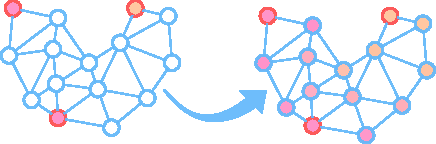
\includegraphics[width=.5\textwidth]{atelier/paradigms/GSSL.pdf}
\end{wrapfigure}

In the semi-supervised learning setting of \cref{sec:PSSL}, we are given a finite set $\domain_n\subset \tilde{\domain}$ consisting of $n$ points, where $\tilde{\domain}$ 
denotes the input space. We assume that a non-empty subset $\conset_n \subset \domain_n$ is labeled, i.e., we are given a labeling function
$\vec g:\conset_n\to\R$. From now on we denote functions acting on a discrete set $\domain_n$ using bold symbols to distinguish them from functions acting onn the continuum $\tilde\domain$. In particular, the space of functions on $\domain_n$ can simply be identified with $\R^n$, since 
 %
\begin{align*}
\{\vec u_n:\domain\to\R\} \sim \R^n.
\end{align*}
%
\noindent%
The semi-supervised learning problem consists in finding an extension of $\vec g$ from $\conset_n$ to the whole set $\domain_n$, i.e.
%
\begin{gather}\label{eq:SSL}
\begin{gathered}\tag{SSL}
\text{find } \vec u:\domain_n\to\R,\\
\text{such that } \vec u(x) = \vec g(x) \text{ for all } x\in\conset_n.
\end{gathered}
\end{gather}
%
%
%
%
In order to obtain meaningful solutions, one usually incorporates the \emph{smoothness assumption} \cite{subramanya2014graph} which can be informally stated as follows:
%
\begin{center}
\enquote{\textit{Points that are close together are more likely to share a similar label.}}
\end{center}
%
%
\paragraph{Weighted Graphs}
In order to employ this assumption we need a notion of \enquote{closeness} on the set $\domain_n$, for which we introduce weighted graphs. Namely we define a weighting function $w$ that allows to compare points in $\domain_n$ and therefore induces the desired notion. 
%
\begin{definition}{Weighted Graphs}{}
For a finite set $\domain_n$ and a weight function $w:V\times V\to\R$, the tuple $(V,w)$ is called a \emph{weighted graph}.
\end{definition}
%
\begin{remark}{}{}
Typically, a graph is defined as a pair $(\domain_n,E)$ where $E$ denotes the set of edges. Here, 
one has two cases:
\begin{itemize}
\item \emph{Undirected graph:} $E=\{ \{x,y\}: \text{there is an edge between } x\in \domain_n \text{ and } y\in \domain_n\}$, i.e., 
$E\subset 2^\domain_n$ and each edge is undirected.
%
\item \emph{Directed graph:} $E=\{ (x,y): \text{there is an edge from } x \text{ to } y\}$, i.e.,
$E\subset \domain_n\times \domain_n$ and each edge is directed.
%
\end{itemize}
Additionally, one then considers a weight function $W:E\to\R$ assigning a weight to each edge, and then defines 
the triple $(\domain_n,E,W)$ as a weighted graph. However, we note that all this information can be represented much more elegantly by a weight function $w:\domain_n\times \domain_n\to\R$. A directed edge set $E\subset \domain_n\times \domain_n$ can be equivalently expressed by 
a weight function $w:\domain_n\times \domain_n\to\R$ where $w(x,y)>0$ if and only if $(x,y)\in E$, a weighting $W:E\to\R$ 
naturally transfers to $w$. In the case of an undirected graph, one simply requires the weight function to be symmetric, i.e., 
$w(x,y)=w(y,x)$ for all $x,y\in \domain_n$.
%
Furthermore, in the above definition the set $\domain_n$ does not enter the definition up to ordering of its $n\in \N$  elements. Therefore, a graph could be entirely represented by a weight function $w:\{1,\ldots,n\}\times\{1,\ldots,n\}\to\R$. However, since the definition of $w$ will incorporate information about points $\domain_n\subset\R^d$ we use the notation $(\domain_n, w_n)$ for graphs in the following.
\end{remark}
%
%
%
\paragraph{The Graph Scale} In most of our applications the data $\domain_n$ is given as a subset of $\R^n$ and in fact we are interested in the limit $n\to\infty$, where $\domain_n$ fills out a domain $\tilde\domain\subset\R^d$. Furthermore, in the continuum we are interested in \emph{local} operators incorporating changes of functions $u:\tilde\domain\to\R$ at an infinitesimal small scale. Since interactions on a graph are inherently non-local in the Euclidean sense, we need to localize the interaction on the graph in the limit $n\to\infty$. A popular choice that guarantees this behavior is to set
%
\begin{align*}
w(x,y) = \eta_{\gscale}(\abs{x-y})
\end{align*}
%
where $\eta_\gscale:[0,\infty)\to [0,\infty]$ is a kernel function depending on a scaling parameter $\gscale\in\R^+$. The parameter $\gscale$ is also referred to as the \emph{graph scale} and informally speaking determines the scale of the graph interactions. I.e., the smaller $\gscale$ the smaller the interaction radius of points in $\domain_n$ should be. In our specific setting of $L^\infty$ problems it is typical to choose
%
%\begin{align*}
%\eta_\gscale(\cdot) = \frac{1}{\c_\eta\ \gscale} \eta\left(\frac{\cdot}{\gscale}\right)
%\end{align*}
%
where $\eta$ is a non-increasing kernel and $c_\eta$ is a constant depending on the kernel.
%
\begin{remark}{}{}
%In the continuum limit one needs to consider the value 
%%
%\begin{align*}
%\sigma_\eta = \sup_{t\in\R^+} t\, \eta(t),
%\end{align*}
%%
%which is assumed to be finite. Considering graph problems in $L^p$ for $p<\infty$
%the corresponding value is given as
%%
%\begin{align*}
%\sigma_\eta^{(p)} = \int_{\R^+} \eta(t)\, t^{d+p} dt
%\end{align*}
%%
%which was first employed in \cite{GarcSlep15} for $p=1$ and then in \cite{slepcev2019analysis} for general $p<\infty$. We see that $\sigma_\eta^{(p)}$ degenerates to $\sigma_\eta$ in the limit $p\to\infty$.
%
%In \cite{roith2022continuum} we choose $c_\eta=1$ and therfore $\sigma_\eta$ then appears in the limit functional. In \cite{bungert2021uniform} we rescale the kernel, i.e., $c_\eta = \sigma_\eta$ which allows to work with unrescaled operators in the limit. 
\end{remark}
%
\section{The $p$-Laplacian: continuum and graph}\label{sec:pLap}
%
In \cref{sec:SSL_Graphs} we explore concepts that borrow ideas from the theory of partial differential equations, and
in particular the $p$-Laplace equation. In this section we briefly review important ideas and results and provide 
necessary preliminaries for the following sections.
%
\subsection{The $p$-Laplacian: continuum setting}\label{sec:pLapcont}
We follow the exposition in \cite{lindqvist2017notes}. Let $\domain\subset\R^d$ be a bounded domain, then 
we consider the $p$-Dirichlet energy for functions $u\in W^{1,p}(\domain)$,
%
\begin{align}\label{eq:DirichletEnergy}
\pDir{}_p(u) := \int_\domain \abs{\Delta_p u}^p \, dx,
\end{align}
%
and the associated variational problem.
%
\begin{problem}{Variational Formulation}{}
For $p\in (1,\infty)$ and $V\subset W^{1,p}(\domain)$ find $u\in W^{1,p}(\domain)$ such that
%
\begin{align*}
\pDir{}_p(u) \leq \pDir{}_p(v)
\end{align*}
%
for all $v$, such that $(u-v)\in W^{1,p}_0$.
\end{problem}
%
If $u\in V$ is a minimizer of the above problem, then its first variation must vanish, i.e., for all $\phi\in C^\infty_0(\domain)$ one has
%
\begin{align}\label{eq:weakLap}
\int_\domain \langle \abs{\Delta_p u}^p \nabla u, \nabla \phi \rangle \, dx = 0.
\end{align}
%
A function $u\in V$ satisfying \cref{eq:weakLap} is called a \emph{weak solution} of the $p$-Laplace equation. In fact, if $u$ 
is smooth enough one has that
%
\begin{align}\label{eq:strongLap}
\Delta_p u := \div(\abs{\Delta_p u}^{p-2} \nabla u) = 0
\end{align}
%
where $\Delta_p$ is called the $p$-Laplacian. For most of our applications we want to prescribe boundary conditions on $\partial \domain$. 
For a given function $g\in W^{1,p}(\domain)$ we therefore consider the set 
$V_g := \{u\in W^{1,p}(\domain): u-g \in W^{1,p}_0(\domain)\}$ for which we have the following result.
%
\begin{theorem}{Existence and Uniqueness}{}
For $p\in (1,\infty)$ and $g\in W^{1,p}(\domain)$ there exists a unique minimizer $u\in V_g$ of the $p$-Dirichlet energy, i.e.,
%
\begin{align*}
\argmin_{u\in V_g} \pDir{}_p(u) = u.
\end{align*}
%
Moreover, $u$ is a weak solution of the $p$-Laplace equation and there exists a function $\tilde{u}\in C(\domain)$ such that
$u = \tilde{u}$ a.e. in $\domain$. If $g\in C(\domain)$ and $\domain$ is sufficiently smooth, then 
$\tilde{u}\vert_{\partial \domain} = g\vert_{\partial \domain}$.
\end{theorem}
%
%
\begin{proof}
The proof can be found in \cite[Thm. 2.16]{lindqvist2017notes}.
\end{proof}
%
%
\paragraph*{Local minimization property}
%
%
\subsection{Laplacian Learning}\label{sec:GpLap}
While there are various techniques to solve the semi-supervised learning problem \eqref{eq:SSL} \cite{}, 
in this work we 
focus on so-called \emph{Laplacian learning} \cite{belkin2006laplacian}. %
This method had one of its first appearances in 
\cite{zhu2003semi}, where the associated problem was given as
%
\begin{gather}\label{eq:SSL_Laplacian}
\begin{gathered}
\min_{\vec u:\domain_n\to\R} \sum_{x,y\in\domain_n} w_n(x,y)^2 
\left(\vec u(y) - \vec u(x) \right)^2\\
\text{subject to } \vec u(x) = \vec g(x) \text{ for all } x\in\conset_n.
\end{gathered}
\end{gather}
%
A natural extension of this problem is obtained by substituting the target functional by
%
\begin{align*}
\GE^{w_n}_p(\vec u):= \sum_{x,y\in\domain_n} w_n(x,y)^p \abs{\vec u(y) - \vec u(x)}^p,
\end{align*}
%
which we refer to as the graph $p$-Dirichlet energy. Indeed, we notice structural 
similarities to the $p$-Dirichlet energy $\pDir_p$ in \cref{eq:DirichletEnergy}, replacing the integral by a finite 
sum and derivatives by weighted finite differences
%
\begin{align*}
 w_n(x,y)^p \abs{\vec u(y) - \vec u(x)}^p.
\end{align*}
%
This naturally leads to the following minimization problem.
%
\begin{problem}{Graph Energy Minimization}{prob:vargraph}
Given a weighted graph $(\domain_n, w_n)$ and a labeling function $\vec g:\conset_n\to\R$, for $\conset_n\subset\domain_n$ we consider 
the problem
%
\begin{align*}
\min_{\vec u:\domain_n\to\R} J^{w_n,p}(\vec u) \text{ subject to } \vec u(x) = \vec g(x) \text{ for all } x\in\conset_n.
\end{align*}
\end{problem}
%
\noindent%
Since every function $\vec u:\domain_n\to\R$ can be identified with a vector $\vec u\in\R^n$, the above problem 
is in fact an optimization problem in $\R^n$. Therefore one can prove unique existence of solutions via standard methods.
%
\begin{theorem}{Existence and Uniqueness}{}
\cref{prob:vargraph} admits a unique solution $\vec u:\domain_n\to\R$.
\end{theorem}
%
\begin{proof}
This and that, a gecko with a hat.
\end{proof}
%
While Laplacian learning 

\paragraph{Graph Laplacian}
%
In the continuum case one considers the Euler--Lagrange equation for the functional $\pDir_p$, which yields the 
$p$-Laplacian, see \cref{sec:pLap}. Analogously, the optimality conditions for the graph $p$-Dirichlet energy $\GE^{w_n}_p$ yield
%
\begin{align*}
\Delta^{w_n}_p \vec u(x):= \sum_{y\in\domain_n} w_n(x,y)^p \abs{\vec u(y) - \vec u(x)}^{p-2} \left( \vec u(y) - \vec u(x) \right) = 0, 
\text{ for all } x\in\domain_n,
\end{align*}
%
where $\Delta^{w_n}_p$ is referred to as thegraph $p$-Laplacian operator. This yields the graph $p$-Laplacian problem.
%
\begin{problem}{Graph $p$-Laplacian}{prob:graphLaplace}
Given a weighted graph $(\domain_n, w_n)$ and a labeling function $\vec g:\conset_n\to\R$ with $\conset_n\subset\domain_n$, find 
a function $\vec u:\domain_n\to\R$ such that
%
\begin{align*}
\Delta_p^{w_n} \vec u &= 0, \text{ in } \domain_n\setminus \conset_n,\\
\vec u &= \vec g \text{ on } \conset_n.
\end{align*}
\end{problem}
%
Since the functional $\GE^{w_n}_p$ has a unique minimizer subject to the constraints given by $\vec g$ and the graph $p$-Laplacian is derived 
via optimality conditions, one expects that the \cref{prob:vargraph} and \cref{prob:graphLaplace} are equivalent. This is formulated in the following 
theorem.
%
\begin{theorem}{Existence and Uniqueness}{}
There exists a unique solution $\vec u:\domain_n\to\R$ to \cref{prob:graphLaplace}, which also is the unique minimizer 
of \cref{prob:vargraph}.
\end{theorem}
%
\begin{proof}
This and that a gecko with a hat.
\end{proof}
%
%
%
%
%
%
%
%
%
%
%
%
%
%
\section{Lipschitz extensions and the infinity Laplacian: continuum and graph}\label{sec:LipExt}
%
%
\subsection{The continuum setting}\label{sec:LipExtCont}
%
%
This chapter studies the limit $p\to\infty$ of the $p$-Laplace equation. We first recall, that for 
$u\in W^{1,\infty}(\domain)$ we have that
%
\begin{align*}
\lim_{p\to\infty} \pDir{}_p(u)^{1/p} = \esssup_{x\in\domain} \abs{\nabla u(x)} =: \pDir{}_\infty(u),
\end{align*}
%
see \cite{jensen1993uniqueness}. The functional $\pDir{}_\infty$ is weak$^*$-lower semicontinuous over $W^{1,\infty}(\domain)$, 
(see e.g. \cite[Thm. 2.6]{barron2001lower}). In the classical theory developed by Jensen in \cite{jensen1993uniqueness} one considers the following problem, which is tries to \enquote{minimize the \emph{sup-norm} of the gradient} as described by Jensen.
%
\begin{problem}{Variational gradient-sup problem}{prob:gradsup}
For an open domain $\domain\subset\R^d$ find a function $u\in W^{1,\infty}(\domain)$ such that
%
\begin{align*}
\norm{\nabla u}_\infty \leq \norm{\nabla v}_\infty \text{ for every } v, \text{s.t. } (u-v)\in W^{1,\infty}_0.
\end{align*}
\end{problem}
%
The above problem becomes more relevant when we additionally impose boundary values $g:\partial\domain\to\R$. Here, \cite{jensen1993uniqueness} draws the connection to so-called \emph{Lipschitz extensions}, which are the driving concept in this section. We introduce a more general viewpoint---that does not require the notion of a gradient---later on, but first introduce the variational problem. 

\paragraph{The intrinsic metric and the Lipschitz constant.}

As noticed in \cite{jensen1993uniqueness} working with the Lipschitz constant and the sup-norm of the gradient requires a careful 
treatment of the distance measurement. Let $\tilde\domain$ be a set and let $d$ be a semi-metric on $\tilde\Omega$, that is $d$ fulfills 
the requirement of a metric up to triangle inequality. Then we define the Lipschitz constant of a function $u:V\to \R$ on a subset $V\subset \tilde\domain$ as
%
\begin{align*}
\Lip_d(u; V):= \sup_{x,y\in V, x\neq y} \frac{\abs{u(x) - u(y)}}{d(x,y)}.
\end{align*}
%
If $d$ denotes the Euclidean distance we use omit the subscript. i.e. $\Lip_d = \Lip$. Additionally, we can 
introduce the space of Lipschitz functions $\Lip_d(V)$ on $V$ via 
$u\in \Lip_d(V) \Leftrightarrow \Lip_d(u;V) <\infty$.
%
\begin{remark}{Lipschitz and Sobolev functions}{}
If $\domain\subset\R^d$ is sufficiently regular, e.g., it has Lipschitz boundary then we have that
%
\begin{align*}
\Lip(\domain) = W^{1,\infty}(\domain),
\end{align*}
%
where this identity is of course to be understood in the sense of equivalence classes in $\L^p$ spaces. We refer to \cite{evansgariepy} for a proof of this result.
\end{remark}
%
The above remark already relates Lipschitz with $W^{1,\infty}$ functions. Often however, we need a quantitative 
comparison between the Lipschitz constant and the sup-norm of the gradient of a function. Here, it is essential 
which distance measure is chosen for the Lipschitz constant. For an open domain $\domain\subset\R^d$ we have the inequality
%
\begin{align*}
\norm{\nabla u}_\infty \leq \sup_{x\neq y} \frac{\abs{u(x) - u(y)}}{\abs{x-y}}
\end{align*}
%
which can be proven via the definition of the gradient. For the reverse inquality, one has to respect the 
geometry of the domain, namely for $x,y\in\domain$ we have that
%
\begin{align}\label{eq:LipGrad}
\abs{u(x) - u(y)} \leq \norm{\nabla u}_\infty\ d_\domain(x,y)
\end{align}
%
see, e.g., \cite[Prop9.3, Rem. 7]{brezis2011functional}, where
%
\begin{align*}
d_\domain(x,y) = \inf \left\{
\int_0^1 \abs{\dot{\gamma}(t)} dt : \gamma\in C^1([0,1], \domain)\text{ with } \gamma(0)=x, \gamma(1) =y
\right\}
\end{align*}
%
denotes the \emph{geodesic distance} on $\domain$. If $\domain$ is convex, we have that $d_\domain(x,y) = \abs{x-y}$ for every 
$x,y\in \domain$ and therefore \cref{eq:LipGrad} yields $\Lip(u) = \norm{\nabla u}_\infty$. However, this situation changes for non-convex domains, see \cref{ex:tube}. Additionally it is often necessary to define 
a distance measure on the closure of $\domain\subset\R^d$. In order to have a geodesic on $\overline{\domain}$ one can simply consider $d_{\overline{\domain}}$, see e.g. \cite{unif}, which then yields the length space $(\overline{\domain}, d_{\overline{\domain}})$. In the classical theory developed in \cite{jensen1993uniqueness} one alternatively considers
%
\begin{align*}
\tilde{d}_{\overline{\domain}}(x,y) := \liminf_{(\tilde x,\tilde y)\to(x,y)} d_\domain(\tilde{x},\tilde{y}).
\end{align*}
%
The differences between these notation are demonstrated in the following example. Also note, that 
$\tilde{d}_{\overline{\domain}}$ is only a semi-metric on $\overline{\domain}$ since it is lacking a 
triangle inequality.
%
\begin{example}{}{ex:tube}
For $I = [-\pi, c]\cup [c, \pi]$ with $c=\pi/6$ we consider the domain
%
\begin{align*}
\bigcup_{\theta \in I} B_1\left((\cos(\theta),\sin(\theta)\right)
\end{align*}
%
which is visualized in \cref{fig:tube} and the points $x=(2\, c, 1), y= (2\, c, -1)$. The 
line segment between $x$ and $y$ contains the point $z=(2\, c, 0)$, however $z\notin \domain$. One can show that 
the geodesic has the length $d_\domain(x,y) = 4\, \cos(\pi/6) + \pi \approx 6.606$ which is the length of the dotted path 
in \cref{fig:tube}. However, we observe that 
%
\begin{align*}
\overline{\domain} = \bigcup_{\theta \in I } 
\overline{B_1\left((\cos(\theta),\sin(\theta)\right)}
\end{align*}
%
and in particular $z\in \overline{B_1\left((c,c)\right)}$, therefore $d_{\overline{\domain}}(x,y) = 2$.
\end{example}
%
\begin{figure}
\centering
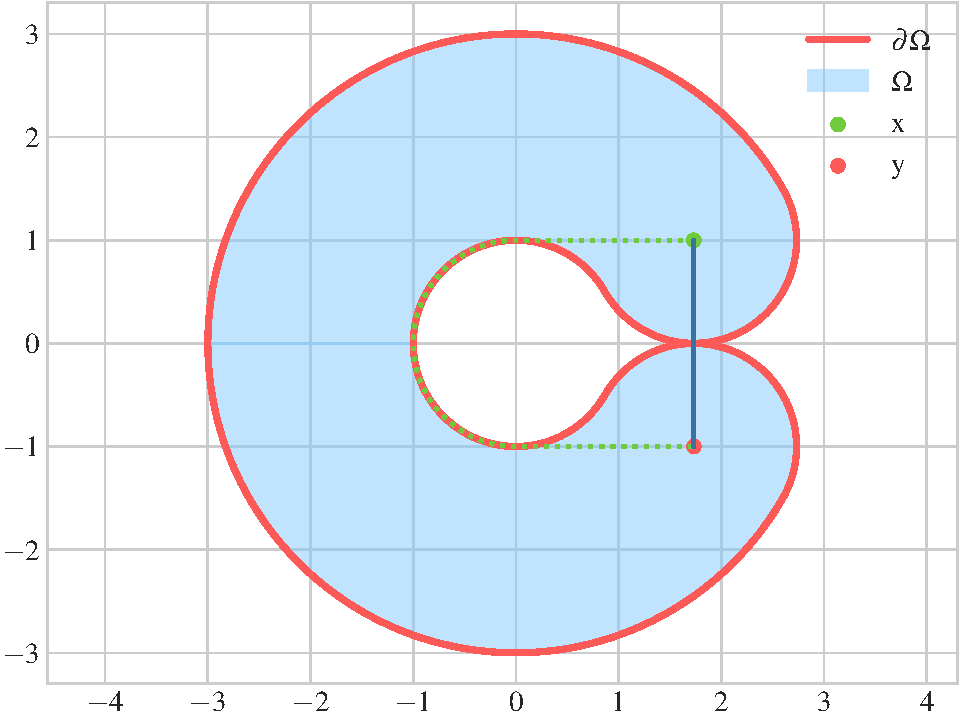
\includegraphics[width=.5\textwidth]{code/domains/tube.pdf}
\caption{The domain in \cref{ex:tube}.}\label{fig:tube}
\end{figure}
%
%
\paragraph{Solutions to the gradient-sup problem}
%
Before generalizing the theory of Lipschitz extension to arbitrary metric spaces, we first note, that one can explicitly construct solutions. Namely, for given $g\in\Lip(\partial\domain)$ the functions 
%
\begin{align}\label{eq:JenSol}
\begin{aligned}
\overline{g}(x) &:= \inf_{y\in\partial\domain} g(y) + 
\Lip_{\tilde{d}_{\overline{\domain}}}(g; \partial\domain)\cdot \tilde{d}_{\overline{\domain}}(x,y)\\
%
\underline{g}(x) &:= \sup_{y\in\partial\domain} g(y) - 
\Lip_{\tilde{d}_{\overline{\domain}}}(g; \partial\domain)\cdot \tilde{d}_{\overline{\domain}}(x,y)
\end{aligned}
\end{align}
%
are solutions to the gradient-sup problem \cref{prob:gradsup} that coincide with $g$ on $\partial\domain$, see \cite[Th. 1.8]{jensen1993uniqueness}.
%
\begin{remark}{}{}
The same concept of constructing solutions is applied in the following sections in a more abstract setting. 
These solutions are then called Whitney and McShane or respectively maximal and minimal extensions, see 
\cref{lem:ext}.
\end{remark}
%
One easily observes that there are cases where $\overline{g}\neq \underline{g}$ and therefore the sup-gradient 
problem does not admit a unique solution. A concrete example, to showcase this phenomena is given  
in \cite[p. 53]{jensen1993uniqueness}.
%
%
\paragraph{Lipschitz extensions in metric spaces}
%
The problem considered in the last section was motivated by a variational problem for $\pDir_\infty(u)=\norm{\nabla u}_\infty$. However, the theory of Lipschitz extensions provides a more general framework. Namely, here we do not assume that $\domain$ is a subset of 
$\R^d$ and rather consider a metric space $(\tilde{\domain},d)$ with $\domain\subset \tilde\domain$. 
%
\begin{remark}{}{}
For applications within this thesis we have that $\domain\subset\R^d$ is an open bounded domain and then consider 
$\tilde\domain:= \closure\domain$, i.e., the closure of $\domain$ within the topology induced by the Euclidean distance. 
In this abstract setting however, we use an abstract space $\tilde\domain$ while still being close notation wise.
\end{remark}
%
%
%
A result originally due to Kierszbraun \cite{Kirszbraun1934} states that for two Hilbert spaces $H_1, H_2$, a subset $\conset\subset H_1$ and a function $g:\conset\to H_1$ there exists a function $u:H_1\to H_2$ such that 
%
\begin{align*}
u &= g \text{ on } U,\\
\Lip(u; H_1) &= \Lip(g; \conset).
\end{align*}
%
Here, the metrics for the respective Lipschitz constants are induced by the inner products of the Hilbert spaces. We refer to \cite{Kirszbraun1934} for the original proof and to \cite[Th. 1.31]{Schwartz1969} for a proof of the version as stated above.
In this work we only consider the case $H_2=\R$ which allows for more general assumption on the space $H_1$. We now formulate the Lipschitz extension problem in our setting.
%
\begin{problem}{Lipschitz Extensions}{prob:Lipext}
Let $(\tilde{\domain},d)$ be a metric space and $\conset\subset \tilde{\domain}$ be a bounded subset. For a given Lipschitz function $g:\conset\to\R$ find a Lipschitz function $u:\tilde\domain\to \R$ such that
%
\begin{align*}
\Lip_d(u; \tilde\domain) = \Lip_d(g; \conset).
\end{align*}
%
A function $u:\tilde{\domain}$ with this property is called \emph{Lipschitz extension} of 
$g$ to $\tilde{\domain}$.
\end{problem}
%
In this setting one can explicitly construct solutions of the Lipschitz extension task. They are not unique, however one has an upper and a lower bound. In fact, conceptually these solutions 
are very similar to the functions in \cref{eq:JenSol} and even coincide, whenever the sup-norm of the gradient is given as the Lipschitz constant.
%
\begin{lemma}{}{lem:ext}
In the setting of \cref{prob:Lipext} we have that the 
%
\begin{itemize}
\item \textbf{Whitney (or maximal) extension:} $\Whit{g}(x) := \inf_{y\in \conset} g(y) + \Lip_d(g; \conset)\cdot d(x,y)$ and the
\item \textbf{McShane (or minimal) extension:} $\McS{g}(x) := \sup_{y\in \conset} g(y) - \Lip_d(g; \conset)\cdot d(x,y)$
\end{itemize}
%
defined for $x\in\tilde\domain$ are Lipschitz extensions of $g$ to $\tilde\domain$. Moreover, let $u:\tilde\domain\to\R$ be any Lipschitz extension of 
$g$, the we have that
%
\begin{align*}
\McS{g} \leq u \leq \Whit{g}.
\end{align*} 
\end{lemma}
%
\begin{proof}
We refer to \cite{whitney1992analytic} and \cite{mcshane1934extension} for the proofs of the respective result.
\end{proof}
%
As demonstrated in \cref{ex:maxprinc}, there are cases where $\Whit{g}\neq\McS{g}$ and 
therefore, Lipschitz extensions are not unique in general. Furthermore, \cite{aronsson2004tour} points out that the Whitney and McShane extension do not allow for a comparison principle, which can also be observed in \cref{ex:maxprinc}.
%
\begin{example}{}{ex:maxprinc}
Consider the set $\tilde\domain = [-1,1]$ and $\conset=\{-1,0,1\}$ with 
%
\begin{align*}
\color{apple}g_1\bc(x)&:= 0,\\
\color{grape}g_2\bc(x)&:= 1/2 (x- \sign(x)\cdot x),\\
\color{sky}g_3\bc(x)&:= -\color{grape}g_2\bc.
\end{align*}
%
Then we have that $\color{grape}g_2\bc\leq \color{apple}g_1\bc$ on $\conset$ but 
%
\begin{align*}
\color{grape}\Whit{g_2}\bc>\color{apple} \Whit{g_1}\bc \text{ in } (0,1),
\end{align*}
%
see \cref{fig:maxprinc} for a visualization. Analogously, we have that $\color{sky}g_3\bc\geq \color{apple}g_1\bc$ on $\conset$ but 
%
\begin{align*}
\color{sky}\McS{g_3}\bc<\color{apple} \McS{g_1}\bc \text{ in } (0,1).
\end{align*}
\end{example}
%
\begin{figure}
\centering
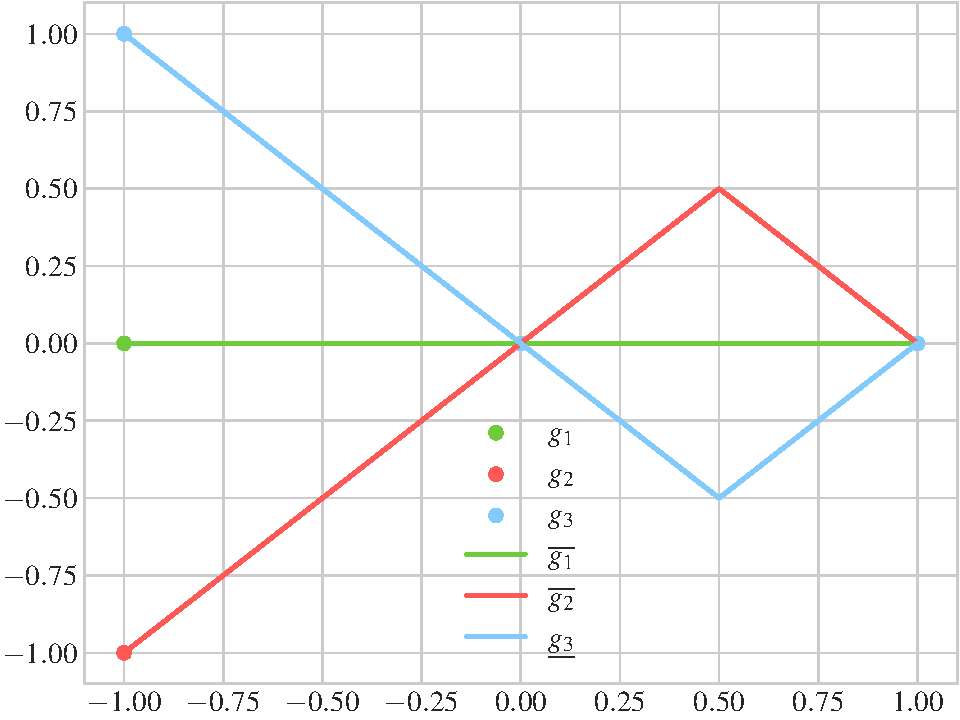
\includegraphics[width=.5\textwidth]{code/lipextcomp/comp.pdf}
\caption{The maximal extension does not admit a comparison principle, as demonstrated in \cref{ex:maxprinc}.}\label{fig:maxprinc}
\end{figure}
%
%
\paragraph{Absolutely Minimizing Extension}\label{sec:AMLE}
%
Sending $p\to\infty$ in the variational formulation of the $p$-Laplace equation 
yields the Lipschitz extension task, which however does not admit for unique solutions. So the question arises, which property is lost in the limit case. For $p<\infty$ one has the crucial local minimization property. Let $\domain\subset\R^d$ be an open domain and denote by $u_p$ the solution of the $p$-Laplace problem with boundary values $g\in W^{1,p}(\domain)$. Then we know that $u_p$ is also a minimizer of $\pDir_p$ on every subset $V\subset \domain$, i.e.,
%
\begin{align*}
\int_V \abs{\nabla u_p}^p dx \leq \int_V \abs{\nabla v}^p dx
\end{align*}
%
for any function $v$ such that $(u_p-v)\in W^{1,p}_0(V)$, see e.g. \cite{}. This lead Aronsson to introduce the concept of \emph{absolutely minimizing Lipschitz extension} in \cite{aronsson1967extension}. A function $u_\infty\in W^{1,\infty}$ is called absolutely minimal, if
%
\begin{align}\label{eq:absmin}
\esssup_{x\in V} \abs{\nabla u} \leq \esssup_{x\in V} \abs{\nabla v} \text{ for every open } V\subset \domain
\end{align}
%
and every function $v$ such that $(u-v)\in W^{1,\infty}_0$. I fact one can also show, that 
$u_p\xrightarrow{p\to\infty} u_\infty$ (\cite{aronsson1967extension}), which seems to validate the notion of absolute minimizers. 
In \cite{tour} it was shown, that one has an equivalent formulation involving the Lipschitz constant. For a given Lipschitz function $f:\overline{\domain}\to\R$ we have that $u_\infty$ with $(u_\infty-f)\in W^{1,\infty}_0(\domain)$ fulfills \cref{eq:absmin} iff
%
\begin{align*}
\Lip(u_\infty; V) \leq \Lip(v; V) \text{ for every } V\subset \domain
\end{align*}
%
and every function $v$ such that $(u-v)\in W^{1,\infty}_0(V)$, see \cite[Th ??]{tour}.\todo{Maybe not Sobolev here}

In this thesis we work with a notion of absolute minimizers, which is equivalent to the above formulation for convex domains in $\R^d$. However, 
$\ldots$
%
\begin{problem}{AMLEs}{prob:amles}
Let $(\tilde{\domain}, d)$ be a length space, $\conset\subset\tilde{\domain}$ a closed subset and $g:\conset\to\R$ a Lipschitz function. Find an extension $u\in C(\tilde{\domain})$ such that $u=g$ on $\conset$ and
%
\begin{align*}
\Lip_d(u; \overline{V}) = \Lip_d(u, \partial V) \text{ for all open and connected sets } V\subset \tilde{\domain}\setminus \conset.
\end{align*}
%
A function $u$ fulfilling this property is called absolutely minimizing Lipschitz extension of $g$.
\end{problem}
%
\begin{remark}{}{}
In our application $\domain$ is an open subset of $\R^d$ and we then choose $\tilde{\domain} = \overline{\domain}$. Here, it is important to note that 
the topological notions like boundary and interior are to be understood relative to $\overline{\domain}$. A visualization odf this concept can be found in \cref{fig:relb}.
\end{remark}
%
\begin{figure}
\begin{center}
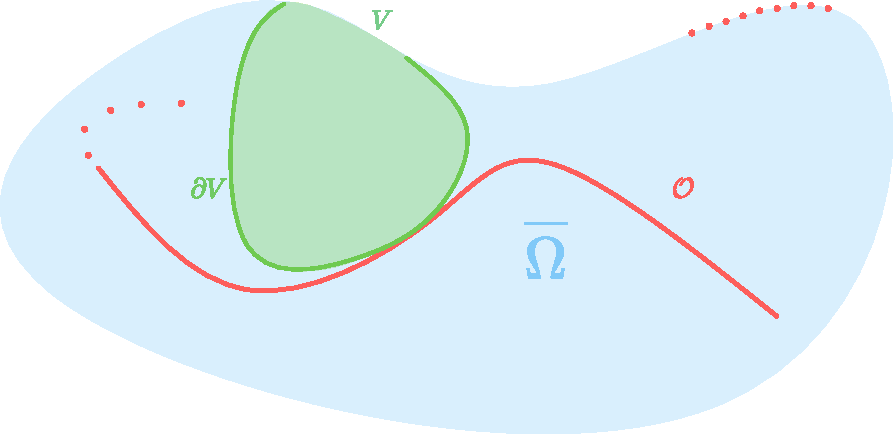
\includegraphics[width=.7\textwidth]{atelier/SSL/relboundary.pdf}
\end{center}
\caption{A set $V\subset\overline{\domain}$ can be relatively open w.r.t. the metric space $\overline{\domain}$ although, $V\cap\partial\domain \neq\emptyset$, where $\partial \domain$ is the boundary within the standard topology on $\R^d$. The relative boundary of $\partial_{\overline{\domain}} V$ does not include any parts of $\partial \domain$.}\label{fig:relb}
\end{figure}
%
%
\paragraph{Comparison with Cones}

\paragraph{The infinity Laplacian}

%
%

\subsection{Graph Lipschitz Extensions}\label{sec:GLipExt}
%
We now consider the limit $p\to\infty$ of \cref{prob:vargraph} in the graph case. Analogously to \cref{sec:InfLip} we derive
%
\begin{align*}
\lim_{p\to\infty} \left(\GE^{w_n}_p(\vec u)\right)^{1/p}= \max_{x,y\in\domain_n} w_n(x,y) \abs{\vec u(y) - \vec u(x)}=:\GE^{w_n}_\infty(\vec u)
\end{align*}
%
which extends the graph $p$-Laplacian energy to the case $p=\infty$. Again we notice structural similarities to 
the continuum version $\pDir_\infty$. 
%
\begin{remark}{}{}
Informally speaking the functional $\GE$ combines elements of a gradient and Lipschitz constant. Assuming that $w_n(x,y)$ relates to $\abs{x-y}$ we see that the finite difference approximation
resembles a Lipschitz constant. However, typically $w_n(x,y)$ has also some localizing property which fits the interpretation of a gradient better.
\end{remark}
%
This functional now leads to the graph Lipschitz extension problem.
%
\begin{problem}{Graph Energy Minimization}{prob:lipgraph}
Given a weighted graph $(\domain_n, w_n)$ and a labeling function $\vec g:\conset_n\to\R$, for $\conset_n\subset\domain_n$ we consider 
the problem
%
\begin{align*}
\min_{\vec u:\domain_n\to\R} \GE_\infty^{w_n}(\vec u) \text{ subject to } \vec u(x) = \vec g(x) \text{ for all } x\in\conset_n.
\end{align*}
\end{problem}
%
\noindent%
Since the weighting function $w_n:\domain_n\times\domain_n\to\R^+_0$ does not induce a metric, \cref{prob:lipgraph} does not directly fit the framework of the abstract Lipschitz Extension in \cref{prob:Lipext}. However, we can consider paths in $(\domain_n, w_n)$, connecting arbitrary $x,y\in\domain_n$ i.e. vectors $\gamma\in\domain_n^{\times k}$ such that 
%
\begin{align*}
w_n(\gamma_i, \gamma_{i+1}) &> 0\quad\text{for all } i=1,\ldots, k-1,\\
\gamma_1 &= x, \\ \gamma_k &= y
\end{align*}
%
for which we define the length as
%
\begin{align*}
\abs{\gamma} = \sum_{i=1}^{k-1} w(\gamma_i, \gamma_{i+1})^{-1}.
\end{align*}
%
This yields the metric space $(\domain_n, d_{w_n})$, where $d_{w_n}:\domain_n\times\domain_n\to\R$ is defined as
%
\begin{align}\label{eq:graphdist}
d_{w_n}(x,y) := \min \left\{ \abs{\gamma}: \gamma \text{ is a path in } 
(\domain_n, w_n)\text{ from } x \text{ to } y\right\}.
\end{align}
%
\begin{remark}{}{}
We note that it is important to only consider non-negative weights, otherwise any loop with a negative \enquote{length} would decrease the 
length of the whole path arbitrarily. However, restricting ourselves to non-negative weights we can easily see, that the minimum in \cref{eq:graphdist} is indeed attained.
\end{remark}
%
With this definition we can consider the Lipschitz extension task of $g:\conset_n\to\R$ to $\domain_n$ within the metric space $(\domain_n,d_{w_n})$, i.e. within the setting of \cref{prob:Lipext}. Therefore the question arises, whether the minimization problem in \cref{prob:lipgraph} is equivalent to the metric Lipschitz extension problem for which we have the following lemma.
%
%
\begin{lemma}{}{}
For a graph $(\domain_n, w_n)$ with non-negative weights and a function $\vec u:\domain_n\to\R$ we have that 
\begin{align*}
\GE_\infty^{w_n}(\vec u) = \Lip_{d_{w_n}}(\vec u).
\end{align*}
%
Furthermore, for $\conset_n\subset\domain_n$ and a function $\vec g:\conset_n\to\R$ and we have that
%
\begin{align*}
\vec g = \vec u \text{ on } \conset_n\Rightarrow
\Lip_{d_{w_n}}(\vec g;\conset_n) \leq \Lip_{d_{w_n}}(\vec u).
\end{align*}
\end{lemma}
%
%
\begin{proof}
\textbf{Step 1:} We show that $\Lip_{d_{w_n}}(\vec u) \leq \GE_\infty^{w_n}(\vec u)$.\\
%
We can choose a path $\gamma\in\domain_n^{\times k}$ such that
%
\begin{align*}
\Lip_{d_{w_n}}(\vec u) &= \frac{\vec u(\gamma_1) - \vec u(\gamma_k)}{\abs{\gamma}}.
\end{align*}
%
The path $\gamma$ allows to compare vertices $\gamma_1, \gamma_k\in\domain_n$ that aren't necessarily neighbors in the graph. However, each consecutive vertices in the path are neighbors in the graph and therefore we have
%
\begin{align}\label{eq:gebound}
w_n(\gamma_i, \gamma_{i+1}) \abs{\vec u(\gamma_{i+1}) - \vec u(\gamma_i)}
&\leq \GE^{w_n}_\infty(\vec u)\quad \text{ for all } i=1,\ldots, k-1.
\end{align} 
%
We now employ an elementary result for numbers $a_i\in\R^+_0, b_i\in\R^+, i=1,\ldots m\in\N$, namely
%
\begin{align}\label{eq:basicineq}
\left[
a_i\cdot b_i \leq c\in\R \quad\text{ for }
i=1,\ldots, m
\right]
%
\Rightarrow 
%
\frac{\sum_{i=1}^{m}a_i}{\sum_{i=1}^{m} b_i^{-1}} \leq c
\end{align}
%
which can be seen as follows
%
\begin{align*}
a_i\cdot b_i &\leq c\quad\text{ for } i=1,\ldots, m\\
\Rightarrow
a_i &\leq b_i^{-1}\cdot c \quad\text{ for } i=1,\ldots, m\\
\Rightarrow\sum_{i=1}^{m} a_i &\leq \left(\sum_{i=1}^m b_i^{-1}\right)\cdot c\\
%
\Rightarrow\frac{\sum_{i=1}^{m} a_i}{\sum_{i=1}^{m} b_i^{-1}} &\leq c.
\end{align*}
%
This then yields 
%
\begin{align*}
\frac{\abs{\vec u(\gamma_1) - \vec u(\gamma_k)}}{\abs{\gamma}}\leq
\frac{\sum_{i=1}^{k-1} \abs{\vec u(\gamma_i) - \vec u(\gamma_{i+1})}}{\abs{\gamma}} = 
\frac{\sum_{i=1}^{k-1} \abs{\vec u(\gamma_i) - \vec u(\gamma_{i+1})}}{\sum_{i=1}^{k-1} w_n(\gamma_i, \gamma_{i+1)^{-1}}}
%
\leq
\GE^{w_n}_\infty(\vec u) 
\end{align*}
%
where in the last inequality we employed \cref{eq:basicineq} together with \cref{eq:gebound}.\\
%
\noindent%
\textbf{Step 2:} We show that $\Lip_{d_{w_n}}(\vec u) \geq\GE_\infty^{w_n}(\vec u)$.\\
%
Let $x,y\in \domain_n$, then we know that $d_w(x,y) \leq w_n(x,y)^{-1}$ and therefore
%
\begin{align*}
\abs{\vec u(x) - \vec u(y)} w_n(x,y)\leq 
\frac{\abs{\vec u(x) - \vec u(y)}}{d_w(x,y)} \leq 
\max_{\bar{x}, \bar{y}\in\domain_n}  
\frac{\abs{\vec u(\bar x) - \vec u(\bar y)}}{d_w(\bar x,\bar y)} = \Lip_{d_{w_n}}(\vec u).
\end{align*}
%
Since this holds for arbitrary $x,y\in\domain_n$ we have that
%
\begin{align*}
\GE^{w_n}_\infty(\vec u) = \max_{x,y\in\domain_n} \abs{\vec u(x) - \vec u(y)} w_n(x,y)
\leq
\Lip_{d_{w_n}}(\vec u).
\end{align*}\\
\noindent%
\textbf{Step 3:} We show that $\Lip_{d_{w_n}}(\vec g;\conset_n) \leq \Lip_{d_{w_n}}(\vec u)$.\\
%
If $\vec g = \vec u$ on $\conset$ this simply follows since the maximum for the Lipschitz constant of $\vec u$ is taken over a larger set. Indeed,

\begin{align*}
\Lip_{d_{w_n}}(\vec u) &= 
\max_{x,y\in\domain_n} \frac{\abs{\vec u(x) - \vec u(y)}}{d_w(x,y)}
\geq 
\max_{x,y\in\conset_n} \frac{\abs{\vec u(x) - \vec u(y)}}{d_w(x,y)}
=
\max_{x,y\in\conset_n} \frac{\abs{\vec g(x) - \vec g(y)}}{d_w(x,y)}\\
&=
\Lip_{d_{w_n}}(\vec u; \conset_n).
\end{align*}
\end{proof}
%
%
%
This lemma shows that the abstract Lipschitz extension task considered on the metric space $(\domain_n, d_{w_n})$ and the Graph $\infty$-Dirichlet minimization task are indeed equivalent. Therefore, we also have the Whitney and McShane extensions
%
\begin{align*}
\Whit{\vec g}(x) &= \inf_{y\in\conset_n} \vec g (y) + d_{w_n}(x,y)\\
\McS{\vec g}(x) &= \sup_{y\in\conset_n} \vec g (y) - d_{w_n}(x,y)
\end{align*}
%
as solutions on the graph. Analogously, the problem does not admit for unique solutions.
%
%
%
\paragraph{Absolutely Minimizing Graph Extensions}
%
Similarly to \cref{sec:AMLE} we can now consider absolutely minimizing extensions. However, the problem in 
\cref{prob:amles} uses a notion of a boundary and it is not directly clear how to infer this concept to the discrete set $\domain_n$. Therefore, we define the following what we mean by \enquote{boundary} on a graph.
%
\begin{definition}{}{}
Let $(\domain_n, w_n)$ be a weight graph and let $V\subset\domain_n$ be a subset, then we define
%
\begin{itemize}
\item the \textbf{exterior} boundary as $\partialext :=\{x\in \domain_n\setminus V: w_n(x,y) > 0 \text{ for some } y\in V\}$,
\item the \textbf{interior} boundary as $\partialint :=\{x\in V: w_n(x,y) > 0 \text{ for some } y\in \domain_n\setminus V\}$.
\end{itemize}
%
The closure of $V$ is then defined as $\extcl{V} V := V\cup \partialext$ and the interior as 
$\stackrel{\circ}{V}^{\text{int}}:= V\setminus \partialint V$.
\end{definition}
%
%
We note that it is not possible to define a topology on $\domain_n$ that would yield the above notions. Namely, the only admissible topology in our case would be the discrete topology, i.e., $2^{\domain_n}$. However, in this topology the only closed sets are $\emptyset$ and $\domain_n$ which is not useful for the applications in the following. Using the Kuratowski closure axioms \cite{kuratowski1922operation} we remark the following.
%
\begin{lemma}{}{}
The exterior closure on a weighted graph $(\domain_n, w_n)$ is a preclosure or Čech closure.
\end{lemma}
%
\begin{proof}
Here, we use the notion of a preclosure in \cite{vcech1966topological}.
We first see that $\overline{\emptyset}^{\text{ext}}=\emptyset$ and that $V\subset \overline{V}^{\text{ext}}$ for every subset $V\subset\domain_n$, i.e. the above defined closure preserves the empty set and is extensive. Furthermore, for two sets $V_1,V_2\subset \domain_n$ we have that
%
\begin{gather*} 
x\in \partialext (V_1\cup V_2)\\
\Leftrightarrow\left[x\notin V_1\cup V_2\right]\wedge \left[\exists y\in V_1\cup V_2: w_n(x,y) \right]\neq 0\\
\Leftrightarrow 
\left[x\notin V_1\cup V_2\right]\wedge
\bigg(\left[\exists y\in V_1: w_n(x,y) \neq 0 \right]\vee
\left[\exists y\in V_2: w_n(x,y) \neq 0 \right]\bigg)\\
\Leftrightarrow \left[x\in \partialext V_1\setminus V_2\right]\vee
\left[x\in  \partialext V_2 \setminus V_1 \right]\\
\Leftrightarrow x\in (\partialext V_1 \cup \partialext V_2)\setminus (V_1\cup V_2).
\end{gather*}
%
We have shown that $\partialext (V_1\cup V_2)=(\partialext V_1 \cup \partialext V_2)\setminus (V_1\cup V_2)$. Therefore, we have that
%
\begin{align*}
\extcl{V_1\cup V_2} &= 
V_1\cup V_2 \cup \partialext (V_1\cup V_2)\\
&= V_1\cup V_2 \cup ((\partialext V_1 \cup \partialext V_2)\setminus (V_1\cup V_2))\\
&= V_1\cup \partialext V_1 \cup V_2 \cup \partialext V_2\\
&= \extcl{V_1}\cup\extcl{V_2}.
\end{align*}
%
This shows that the closure preserves binary unions and therefore we have shown, that it is indeed a Čech closure.
\end{proof}
%
%
%
The missing property, that inhibits the closure to induce a topology is the so-called idempotence. Namely, there are sets $V\subset \domain_n$ such that
%
\begin{align*}
\overline{V}^{\text{ext}} \neq \extcl{\extcl{V}}.
\end{align*}
%
\begin{figure}
\centering
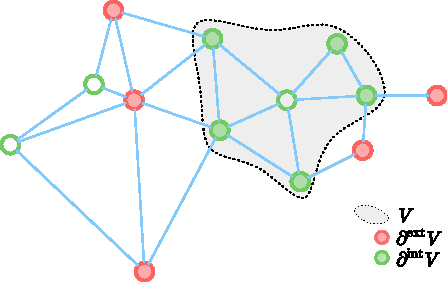
\includegraphics{atelier/SSL/boundary.pdf}
\caption{Visualization of exterior and interior boundary on a graph.}\label{fig:graphb}
\end{figure}
%
E.g. in the example visualized in \cref{fig:graphb} we see that $\overline{\overline{V}^{\text{ext}}}^{\text{ext}}=\domain_n\neq \overline{V}^{\text{ext}}$. Since the closure we employ here does not induce a topology, we have a slightly modified notion of absolutely minimizers.
%
\begin{problem}{Graph AMLEs}{prob:GAMLE}
Given a connected weighted graph $(\domain_n, w_n)$, $\conset_n\subset\domain_n)$ and a function $\vec g:\conset_n\to\R$ find a function $\vec u:\domain_n\to\R$ such that
%
\begin{align*}
\Lip_{d_{w_n}}(\vec u; \extcl{V}) &= \Lip_{d_{w_n}}(\vec u; \partialext V)
\text{ for all connected } V\subset \domain_n\setminus\conset_n,\\
\vec u &= \vec g\text{ on } \conset_n.
\end{align*}
\end{problem}
%
%
%
\paragraph{Comparison with graph Distance functions}
%
Analogously to the continuum case \cref{??} we can also consider comparison with distance functions on graphs. The main ingredients here, are the graph distance function $d_{w_n}$ and the notion of closure on a graph as developed in the last section.
%
%
\begin{definition}{}{}
For a weighted graph $(\domain_n,w_n)$ we say a function $\vec u:\domain_n\to\R$ fulfills comparison with distance function from above (CDFA) on a subset $U\subset \domain_n$ if for every $V\subset U$ we have
%
\begin{align}\label{eq:CDFA}\tag{CDFA}
\max_{\extcl{V}} \left(u + a\ d_{w_n}(\cdot, z)\right)=
\max_{\partialext V} \left(u + a\ d_{w_n}(\cdot, z)\right)
\end{align}
%
for every $z\in \domain_n\setminus V$ and every $a\in\R$. We say that $\vec u$ fulfills comparison with distance function from below (CDFB) on a subset $U\subset \domain_n$ if for every $V\subset U$ we have
%
\begin{align}\label{eq:CDFB}\tag{CDFB}
\min_{\extcl{V}} \left(u - a\ d_{w_n}(\cdot, z)\right)=
\min_{\partialext V} \left(u - a\ d_{w_n}(\cdot, z)\right)
\end{align}
%
for every $z\in \domain_n\setminus V$ and every $a\in\R$.
\end{definition}
%
%
Analogously to the continuum case, we say that a function fulfills comparison with distance functions, if it fulfills both, \cref{eq:CDFA} and \cref{eq:CDFB}. Existence of such functions is established later, we are first interested in the question of uniqueness. Since the notion of graph boundaries is not directly compatible with the usual definitions on metric spaces, we prove it separately. Here, we adapt arguments from [smart] and [LeGruyer]. To do so we first consider the operators
%
\def\eps{\varepsilon}
\begin{align*}
\vec S^\eps \vec u (x) := \max_{y\in\domain_n: d_{w_n}(x,y)\leq \eps} \vec u(y) \quad
\vec S_\eps \vec u (x) := \min_{y\in\domain_n: d_{w_n}(x,y)\leq \eps} \vec u(y)
\end{align*}
%
and proof the following lemma, which is the analogue of 

%
%
%
%
\paragraph{The Graph infinity Laplacian}
%
We can also obtain the limit of the Graph $p$-Laplace operator via the following formal calculation,
%
\begin{align*}
\Delta^{w_n}_p \vec u(x) &= 0\\
\Leftrightarrow \sum_{y\in\domain_n} w_n(x,y)^{p} \abs{\vec u(y) - \vec u(x)}^{p-2} (\vec u(y) - \vec u(x)) &= 0\\
%
\Leftrightarrow 
\sum_{y: \vec u(x)\leq \vec u(y)} w_n(x,y)^{p}(\vec u(y)-\vec u(x))^{p-1}
&= \sum_{y: \vec u(x)> \vec u(y)} w_n(x,y)^{p}(\vec u(x)-\vec u(y))^{p-1}.
%\\
%\Leftrightarrow
%\left(\sum_{y: \vec u(x)\leq \vec u(y)} w_n(x,y)^{p}(\vec u(y)-\vec u(x))^{p-1}\right)^{1/p}
%&=\\
%\left(\sum_{y: \vec u(x)> \vec u(y)} w_n(x,y)^{p}(\vec u(x)-\vec u(y))^{p-1}\right)^{1/p}
\end{align*}
%
Taking the terms on the left and right hand side to the power of $1/p$ and then formally sending $p\to\infty$ then yields
%
\begin{align*}
\max_{y: \vec u(x)\leq \vec u(y)} w_n(x,y)(\vec u(y)-\vec u(x)) &= 
\max_{y: \vec u(x) > \vec u(y)} w_n(x,y)(\vec u(x)-\vec u(y))\\
%
\Leftrightarrow \max_{y\in\domain_n} w_n(x,y)(\vec u(y)-\vec u(x)) &= 
-\min_{y\in\domain_n} w_n(x,y)(\vec u(y)-\vec u(x)).
\end{align*}
%
%
This calculation motivates the definition of the graph infinity Laplacian
%
\begin{align*}
\Delta_\infty^{w_n} \vec u(x) := \max_{y\in\domain_n} w_n(x,y)(\vec u(y)-\vec u(x)) +
\min_{y\in\domain_n} w_n(x,y)(\vec u(y)-\vec u(x)),
\end{align*}
%
which then allows to formulate the associated problem as an  extension of \cref{prob:graphLaplace}.

\begin{problem}{Graph $\infty$-Laplacian}{prob:graphinfLaplace}
Given a weighted graph $(\domain_n, w_n)$ and a labeling function $\vec g:\conset_n\to\R$ with $\conset_n\subset\domain_n$, find 
a function $\vec u:\domain_n\to\R$ such that
%
\begin{align*}
\Delta_\infty^{w_n} \vec u &= 0, \text{ in } \domain_n\setminus \conset_n,\\
\vec u &= \vec g \text{ on } \conset_n.
\end{align*}
\end{problem}
%
%
This problem is again well-posed, which is formulated in the following lemma.
%
\begin{lemma}{}{}
There exists a unique solution for \cref{prob:graphinfLaplace}.
\end{lemma}
%
%
\paragraph{Relation between the Graph Lipschitz Extensions}
We now establish the connection between the different notions of Lipschitz extensions. Compared to the continuum case we do not establish the full equivalences but only the necessary implications required for the convergence proofs in \cite{bungert2021uniform}.

First we see, that graph AMLEs are indeed special solutions of the basic Lipschitz extension problem on the graph.
%
\begin{lemma}{}{}
A graph AMLE is also a Lipschitz extension.
\end{lemma}
%
\begin{proof}

\end{proof}
%
%
We now state the main result concerning the relation between the graph infinity Laplacian, graph AMLEs and comparison cones.
%
%
\begin{lemma}{}{}
Let $(\domain_n,w_n)$ be a weighted connected graph and $\vec g:\conset_n\to\R$ be a given function for $\conset_n\subset\domain_n$. Furthermore, let $\vec u:\domain_n\to\R$ be graph infinity harmonic on $\domain_n\setminus\conset_n$ with boundary conditions given by $\vec g$, i.e., $\vec u$ solves \cref{prob:graphinfLaplace} then we have that
%
\begin{itemize}
\item $\vec u$ is an graph AMLE, i.e., $\vec u$ solves \cref{prob:GAMLE},
\item $\vec u$ fulfills comparison with cones.
\end{itemize}
\end{lemma}
%
%
\begin{proof}
Both of the stament are proven in \cite{bungert2021uniform}. From \cite[Prop. 3.8]{bungert2021uniform} we have that $\vec u$ is an graph AMLE. Furthermore, form \cite[Th. 3.2]{bungert2021uniform} we have that $\vec u$ fulfills comparison with cones. In fact, \cite[Th. 3.2]{bungert2021uniform}, shows a more refined statement, namely that
%
\begin{align*}
-\Delta^{w_n}_\infty \vec u &\leq 0 \Rightarrow \vec u \text{ fulfills CDFA},\\
-\Delta^{w_n}_\infty \vec u &\geq 0 \Rightarrow \vec u \text{ fulfills CDFB}.
\end{align*}
%
\end{proof}


\section{Gamma Convergence}\label{sec:GConv}
%
\section{Ratio Convergence}\label{sec:RatConv}
%

